% arara: pdflatex: {action: nonstopmode}

\documentclass[a4paper, 11pt]{scrreprt}

\usepackage[utf8]{inputenc}
\usepackage[english]{babel}
\usepackage[pdftex]{graphicx}
\usepackage{longtable,tabu}
\usepackage[bookmarks=true]{hyperref}
\usepackage{amsmath}
\usepackage{multirow}
\usepackage{rotating}
\usepackage{pdfpages}
\usepackage{float}
%\usepackage{multicolumn}

\hypersetup{
    bookmarks=false,    % show bookmarks bar?
    pdftitle={System Design},    % title
    pdfauthor={Pascal Grosch},                     % author
    pdfsubject={Design: Recording of Tests for Autonomous Vehicles},                        % subject of the document
    pdfkeywords={testing, autonomous vehicle, bachelor thesis, design, recording}, % list of keywords
    colorlinks=true,       % false: boxed links; true: colored links
    linkcolor=black,       % color of internal links
    citecolor=black,       % color of links to bibliography
    filecolor=black,        % color of file links
    urlcolor=purple,        % color of external links
    linktoc=page            % only page is linked
}%

\title{%
\flushright
\rule{16cm}{5pt}\vskip1cm
\Huge{SOFTWARE DESIGN}\\
\vspace{2cm}
for\\
\vspace{2cm}
Recording System for Scenarios for Autonomous Vehicles\\
\vfill
\rule{16cm}{5pt}
}
\date{}

\usepackage{hyperref}

\graphicspath{
  {./images/}
}

\tabulinesep=1.5mm

%!TeX root=./DesignDocument.tex

\newcounter{scenarioCounter}[section]

\newcounter{stepCounter}[scenarioCounter]

\newenvironment{scenario}{
	\newcommand{\step}[1]{
		\multicolumn{6}{|l|}{\textbf{Situation \thestepCounter:} ##1}\\ \hline
		\stepcounter{stepCounter}
	}
	\newcommand{\scenarioItem}[6]{
		##1 & ##2 & ##3 & ##4 & ##5 & ##6\\ \hline
	}
	\begin{longtabu}{|X[-1,m, l]||X[-1,r,m]|X[-1,r,m]|X[-1,r,m]|X[-1,r,m]|X[-1,l,r,m]|}
	\hline
	\rowfont[c]{\bfseries} VehID  & RelX & RelV & Lane & Acc & LnChg\\ \hline
	\step{Initial Situation}
}{
	\end{longtabu}
	\stepcounter{scenarioCounter}
}

\makeatletter
\def\@cline#1-#2\@nil{%
  \omit
  \@multicnt#1%
  \advance\@multispan\m@ne
  \ifnum\@multicnt=\@ne\@firstofone{&\omit}\fi
  \@multicnt#2%
  \advance\@multicnt-#1%
  \advance\@multispan\@ne
  \leaders\hrule\@height\arrayrulewidth\hfill
  \cr
  \noalign{\nobreak\vskip-\arrayrulewidth}}
\makeatother

\begin{document}
	\maketitle
	\tableofcontents
	
	\chapter{System Architecture}
	\section{Component Diagram}
		
		\begin{figure}[H]
			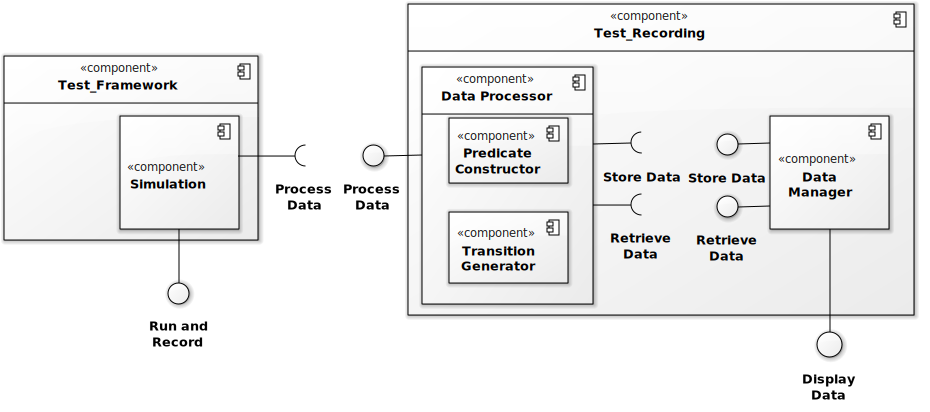
\includegraphics[width=\textwidth]{ComponentDiagram}
			\caption{Component Diagram}
		\end{figure}
	
	\section{Component Description}
	
		\begin{longtabu}{|X[-1,m]|X[l,m]|}
			\hline
			\rowfont[l]{\bfseries} Component Name & Description \\ \hline
			Simulation & The Simulation component executes the actual simulation, filters out irrelevant objects and passes the raw data to the Data Processor.\\ \hline
			Data Processor & The Data Processor component takes raw data, uses hysteresis to transform it to predicates and then stores it in the Data Manager. The second function of the Data Processor component is to retrieve the stored data and condense sequences of situations.\\ \hline
			Predicate Constructor & The Predicate Constructor component uses hysteresis to transform raw data to predicates\\ \hline
			Transition Generator & The Transition Generator compares the current situation with the new data and creates a transition if necessary.\\ \hline
			Data Manager & The Data Manager component wraps the actual data storage and transforms the data between the format of the system and the format of the data storage.\\ \hline
			\caption{Component Description}
		\end{longtabu}
	
	\section{Interface Description}

	\begin{longtabu}{|X[-1,m]|X[l,m]|}
		\hline
		\rowfont[l]{\bfseries} Interface Name & Description \\ \hline
		Run and Record & This interface provides methods to run the simulation while recording the data.\\ \hline
		Process Data & This interface provides methods to take data and process it according to the requirements.\\ \hline
		Display Data & This interface provides methods to use the stored data to create visual representations of the situation graph.\\ \hline
		Store Data & This interface provides methods to transform data from the system format to the data storage format and store them.\\ \hline
		Retrieve Data & This interface provides methods to retrieve data from the data storage and transform it to the system format.\\ \hline
		\caption{Interface Description}
	\end{longtabu}
	
	\chapter{Data}
	\section{Data Flow Diagram}
		
		\begin{figure}[H]
			\centering
			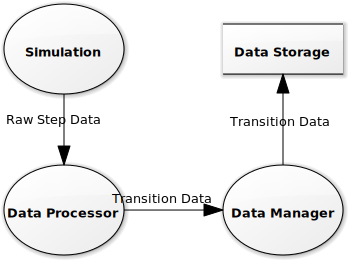
\includegraphics[width=0.5\textwidth]{DataFlowDiagramSystem}
			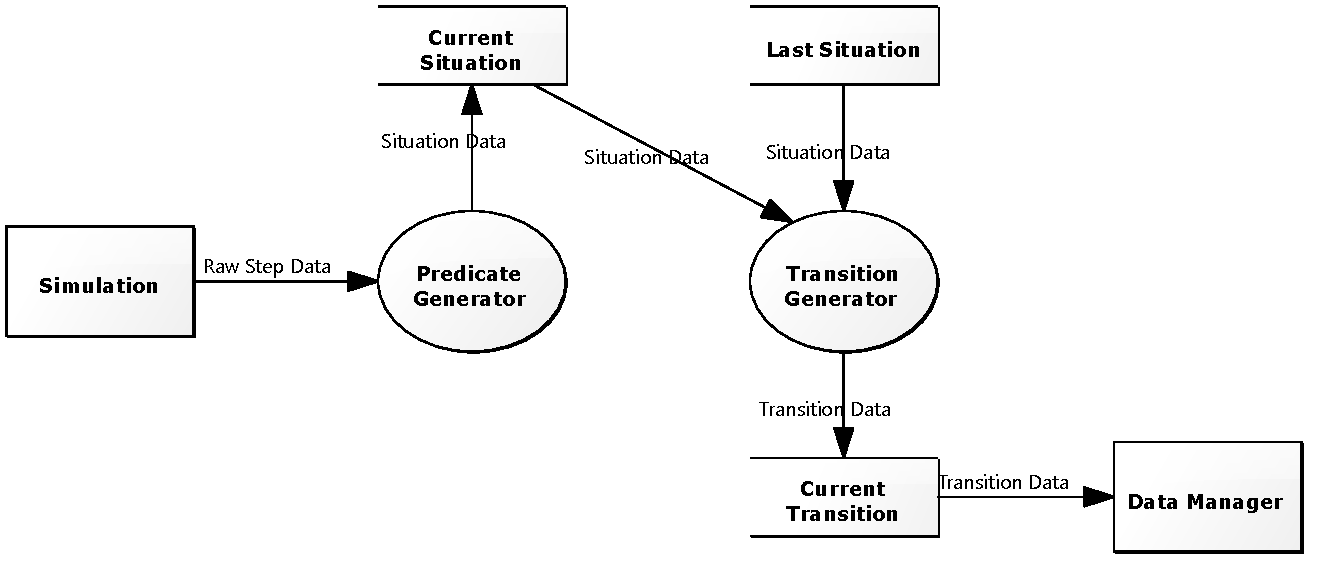
\includegraphics[width=\textwidth]{DataFlowDiagramDataProcessor}
			\caption{Data Flow Diagram on system level on on Data Processor level}
			\label{fig:data_flow_diagram_record}
		\end{figure}
		
	\section{Data Description}

	\begin{longtabu}{|X[-1,m]|X[l,m]|}
		\hline
		\rowfont[l]{\bfseries} Data & Description \endhead \hline
		Raw Step Data & Contains for each relevant vehicle
			\begin{itemize}
				\item velocity $\left[\frac{\text{km}}{\text{h}}\right]$
				\item x-position on the link $\left[m\right]$
				\item lane-number of the current lane starting with 1 on the right
				\item acceleration $\left[\frac{\text{m}}{\text{s$^2$}}\right]$
				\item lane-change indicator ($0$=none, $1$=left, $-1$=right)
				\item desired velocity $\left[\frac{\text{km}}{\text{h}}\right]$
				\item lane-number of the desired lane starting with 1 on the right
			\end{itemize} 
			and is sent in every simulation step.\\ \hline
		Situation Data & Contains Predicate values for the variables listed in table \ref{tab:predicate_variables} for the VUT and other vehicles.\\ \hline
		Transition Data & Contains Situation Data of the predecessor and successor situation.\\ \hline
		\caption{Data Description}
		\label{tab:data_description}
	\end{longtabu}
	
	\subsection{Variables and Values}		
		\begin{longtabu}{|X[-1,l,m]|X[l,m]|X[l,-1,m]|X[-1,l,m]|X[l,m]|}
			\hline
			\rowfont[l]{\bfseries} \shortstack[l]{Related Object} & Category Variable(ID-Short-Name) Number Categories & ID & \multicolumn{2}{l|}{Values}\endhead \hline
			\multirow{5}{\linewidth}{Vehicle} & \multirow{5}{*}{\shortstack[l]{Relative x position of\\the other vehicle to\\the VUT\\(Relx - 1020)\\$d:$ distance$[m]$,\\$v:$ velocity$\left[\frac{km}{h}\right]$\\Num: 5}} & 102030 & [- -] & The other vehicle is behind ($\frac{d}{v} < -1.0$) \\* \cline{3-5}
			& & 102040 & [-] & The other vehicle is close behind ($-1.25<\frac{d}{v} < -0.25$)\\* \cline{3-5}
			& & 102050 & [0] & The other vehicle is on the same height ($-0.5 < \frac{d}{v} < 0.5$)\\* \cline{3-5}
			& & 102060 & [+] & The other vehicle is close in front ($0.25 < \frac{d}{v} < 1.25$)\\* \cline{3-5}
			& & 102070 & [++] & The other vehicle is in front ($1.0 < \frac{d}{v}$)\\ \hline
			& & & & \\
			\multirow{3}{\linewidth}{Vehicle} & \multirow{3}{*}{\shortstack[l]{Relative velocity $v_{rel}$\\of the other vehicle\\to the VUT\\(RelV - 1030)\\Num: 3}} & 103040 & [-] & slower ($v_{rel} < 0.9$)\\* \cline{3-5}
			& & 103050 & [0] & same ($0.75 < v_{rel} < 1.25$)\\* \cline{3-5}
			& & 103060 & [+] & faster ($v_{rel} > 1.1$)\\ \hline
			\multirow{3}{\linewidth}{Vehicle} & \multirow{3}{\linewidth}{Number of Lane} & 104010 & 1 & very right lane\\* \cline{3-5}
			& & 104020 & 2 & middle\\* \cline{3-5}
			& & 104030 & 3 & left\\ \hline
			\multirow{3}{\linewidth}{Vehicle} & \multirow{3}{*}{\shortstack[l]{Acceleration response\\of the VUT\\(Acc - 1050)\\$a:$ acceleration $[\frac{m}{s^2}]$}} & 105040 & [-] & The VUT is braking ($a<-1$)\\* \cline{3-5}
			& & 105050 & [0] & No acceleration ($-2 < a < 2$)\\* \cline{3-5}
			& & 105060 & [+] & The VUT is accelerating ($1 < a$)\\ \hline
			\multirow{3}{\linewidth}{Vehicle} & \multirow{3}{*}{\shortstack[l]{Lane change response\\of the VUT\\(LnChg - 1060)\\$cl:$ current lane\\$nl:$ next lane}} & 106040 & [-] & lane change right ($nl < cl$)\\* \cline{3-5}
			& & 106050 & [0] & No lane change ($nl = cl$)\\* \cline{3-5}
			& & 106060 & [+] & lane change left ($nl > cl$)\\ \hline
			\caption{Predicate variables and values}
			\label{tab:predicate_variables}
		\end{longtabu}
	\newpage
	\section{Data Storage}
	
		
	
	\subsection{Database Schema}
		
		\begin{figure}[H]
		\centering
		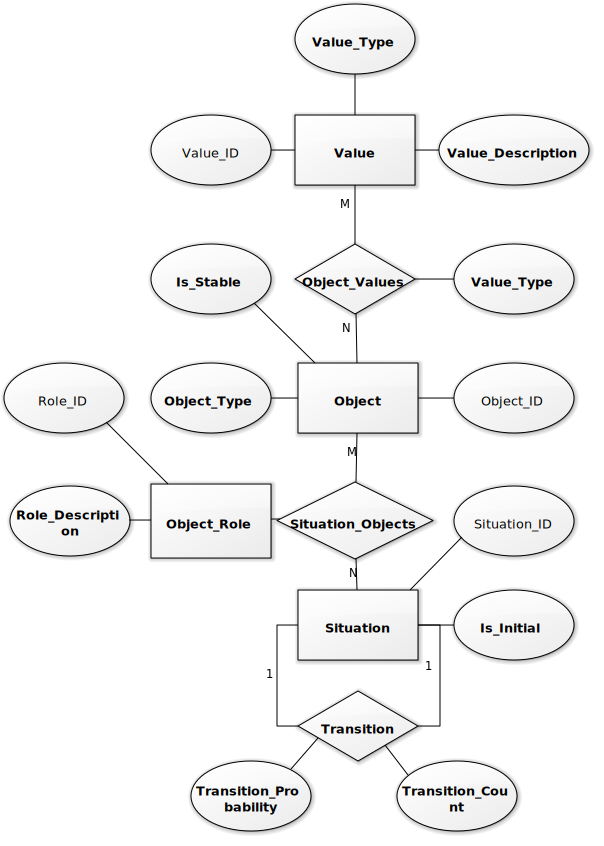
\includegraphics[width=0.74\textwidth]{DatabaseSchema}
		\caption{Entity-Relationship-Diagram}
		\label{fig:er_diagram}
		\end{figure}

	\chapter{Optimization}
	\section{Sight Range}
		
		\begin{figure}
			\centering
			\def\svgwidth{\textwidth}
			\input{./images/distances.pdf_tex}
			\caption{Visualization of the distance classes.}
			\label{fig:view_distances}
		\end{figure}
		
		To avoid collecting unnecessary data or omitting important data the range in which vehicles are considered for data collection is chosen dependent on the current velocity of the vehicle under test.
		Since distance distributions in Vissim are objects that need to be specified before running the simulation classes of ranges are defined beforehand.
		They are chosen by the length of a velocity interval and a factor for the distance in meter (see figure \ref{fig:view_distances}.
		The velocity range is chosen as $v=40\frac{km}{h}$ and the factor is chosen as $d=2.5$ to cover 5 times the recommended safety distance.
		The maximum velocity is chosen as $240\frac{km}{h}$ which results in 7 distance classes.
		Those classes can be seen in table \ref{tab:view_distances}.
		
		\begin{longtabu}{|X[-1,m]|X[-1,m]|}
			\hline
			\rowfont[l]{\bfseries} Velocity Interval[$\frac{km}{h}$] & Sight Distance[$m$]\endhead\hline
			$0 \leq v < 40$ & 100\\ \hline
			$40 \leq v < 80$ & 200\\ \hline
			$80 \leq v < 120$ & 300\\ \hline
			$120 \leq v < 160$ & 400\\ \hline
			$160 \leq v < 200$ & 500\\ \hline
			$200 \leq v < 240$ & 600\\ \hline
			$240 \leq v$ & 700\\ \hline
			\caption{Distance classes}
			\label{tab:view_distances}
		\end{longtabu}
		
		A drawback of this method of observation is the omitting of vehicles which are arriving with a much higher velocity from behind.
		Since this project does not consider traffic jams or crashes this situation can be omitted.
		
	\section{Concurrency}
		
		To Optimize the runtime of the system the simulation and data analysis should run concurrent.
		To retain the correct order of data delivered by the simulation a synchronized queue and the producer-consumer pattern is used.
		
	\chapter{Examples of Expected Scenarios}
	%!TeX root=./DesignDocument.tex


%\scenarioItem{ID}{RelX}{RelV}{Lane}{Acc}{LnChg}

\begin{scenario}
	\scenarioItem{0}{102050}{103050}{1}{105050}{106050}
	
	\step{Slower vehicle in front appears}
	\scenarioItem{0}{102050}{103050}{1}{105050}{106050}
	\scenarioItem{1}{102070}{103040}{1}{105050}{106050}
	
	\step{VUT gets closer to vehicle 1}
	\scenarioItem{0}{102050}{103050}{1}{105050}{106050}
	\scenarioItem{1}{102060}{103040}{1}{105050} {106050}
	
	\step{VUT breaks}
	\scenarioItem{0}{102050}{103050}{1}{105040}{106050}
	\scenarioItem{1}{102060}{103040}{1}{105050}{106050}
	
	\step{VUT follows vehicle 0}
	\scenarioItem{0}{102050}{103050}{1}{105050}{106050}
	\scenarioItem{1}{102060}{103050}{1}{105050} {106050}
\end{scenario}

\begin{scenario}
	\scenarioItem{0}{102050}{103050}{1}{105050}{106050}
	
	\step{Faster vehicle appears behind the VUT on the left lane}
	\scenarioItem{0}{102050}{103050}{1}{105050}{106050}
	\scenarioItem{1}{102030}{103060}{2}{105050}{106050}
	
	\step{Faster vehicle approaches VUT}
	\scenarioItem{0}{102050}{103050}{1}{105050}{106050}
	\scenarioItem{1}{102040}{103060}{2}{105050}{106050}
	
	\step{Faster vehicle overtakes VUT}
	\scenarioItem{0}{102050}{103050}{1}{105050}{106050}
	\scenarioItem{1}{102050}{103060}{2}{105050}{106050}
	
	\step{Faster vehicle moves away}
	\scenarioItem{0}{102050}{103050}{1}{105050}{106050}
	\scenarioItem{1}{102060}{103060}{2}{105050}{106050}
	
	\step{Faster vehicle moves away}
	\scenarioItem{0}{102050}{103050}{1}{105050}{106050}
	\scenarioItem{1}{102070}{103050}{2}{105050}{106050}
	
	\step{Faster vehicle leaves the visible range}
	\scenarioItem{0}{102050}{103050}{1}{105050}{106050}
\end{scenario}

\begin{scenario}
	\scenarioItem{0}{102050}{103050}{1}{105050}{106050}
	
	\step{Slower vehicle in front appears}
	\scenarioItem{0}{102050}{103050}{1}{105050}{106050}
	\scenarioItem{1}{102070}{103040}{1}{105050}{106050}
	
	\step{VUT gets closer to vehicle10}
	\scenarioItem{0}{102050}{103050}{1}{105050}{106050}
	\scenarioItem{1}{102060}{103040}{1}{105050} {106050}
	
	\step{VUT changes lane to the left}
	\scenarioItem{0}{102050}{103050}{1}{105050}{106060}
	\scenarioItem{1}{102060}{103040}{1}{105050}{106050}
	
	\step{VUT completed lane change}
	\scenarioItem{0}{102050}{103050}{2}{105050}{106050}
	\scenarioItem{1}{102060}{103040}{1}{105050}{106050}
	
	\step{VUT is on the same height}
	\scenarioItem{0}{102050}{103050}{2}{105050}{106050}
	\scenarioItem{1}{102060}{103050}{1}{105050}{106050}
	
	\step{VUT is close in front}
	\scenarioItem{0}{102050}{103050}{2}{105050}{106050}
	\scenarioItem{1}{102060}{103060}{1}{105050}{106050}
	
	\step{VUT changes lane to the right}
	\scenarioItem{0}{102050}{103050}{2}{105050}{106040}
	\scenarioItem{1}{102060}{103060}{1}{105050}{106050}
	
	\step{VUT completed lane change}
	\scenarioItem{0}{102050}{103050}{1}{105050}{106050}
	\scenarioItem{1}{102060}{103060}{1}{105050}{106050}
\end{scenario}	
	
	\chapter{Traceability}
		
		\begin{tabu}{|>{\bfseries}X[l,m]|X[-1,c,m]|X[-1,c,m]|X[-1,c,m]|X[-1,c,m]|X[-1,c,m]|X[c,-1,m]|X[c,-1,m]|}
			\hline
			\rowfont[l]{\bfseries} & SF10 & SF20 & SF30 & SF40 & SF50 & SF60 & SF70\\ \hline
			Simulation & X & & & & & & \\ \hline
			Data Processor & & X & & & & &\\ \hline
			Predicate Constructor & & & X & & & X &\\ \hline
			Transition Generator & & & & X & & & \\ \hline
			Data Manager & & & & & X & & X\\ \hline
		\end{tabu}
\end{document}